\documentclass[11pt,letterpaper]{article}
\usepackage[lmargin=1in,rmargin=1in,tmargin=1in,bmargin=1in]{geometry}
\usepackage{../style/homework}
\setbool{quotetype}{false} % True: Side; False: Under
\setbool{hideans}{true} % Student: True; Instructor: False

% -------------------
% Content
% -------------------
\begin{document}

\homework{12: Due 03/20}{Mitchell's mother has a problem\dots with me. Last Christmas, for example. She gave me a piece of exercise equipment and a lettuce dryer. So, to recap, I gave her a gorgeous pair of diamond earrings and she gave me a hint.}{Cameron Tucker, Modern Family}

% Problem 1
\problem{10} Find the equation of the line plotted below.
	\[
	\fbox{
	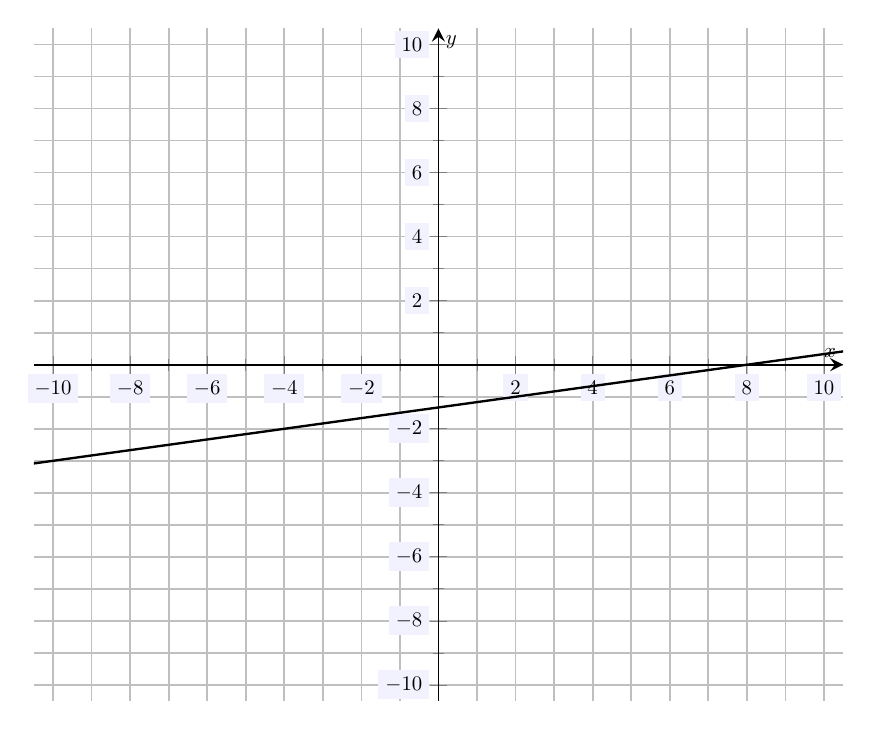
\begin{tikzpicture}[scale=1.5,every node/.style={scale=0.5}]
	\begin{axis}[
	grid=both,
	axis lines=middle,
	ticklabel style={fill=blue!5!white},
	xmin= -10.5, xmax=10.5,
	ymin= -10.5, ymax=10.5,
	xtick={-10,-8,-6,-4,-2,0,2,4,6,8,10},
	ytick={-10,-8,-6,-4,-2,0,2,4,6,8,10},
	minor tick = {-10,-9,...,10},
	xlabel=\(x\),ylabel=\(y\),
	]
	\addplot[line width= 0.02cm,samples=2,domain= -10.5:10.5] ({x},{-4/3 + 1/6*x});
	\end{axis}
	\end{tikzpicture}
	}
	\] 



\newpage



% Problem 2
\problem{10} Find the equation of the following lines:
	\begin{enumerate}[(a)]
	\item The line through $(-1, 1)$ and $(6, -2)$.
	\item The line containing $(8, -1)$ with slope $\frac{4}{3}$.
	\item The line with $y$-intercept 5 and slope $-6$.
	\end{enumerate}



\newpage



% Problem 3
\problem{10} Find the equation of the line with $x$-intercept $-4$ and $y$-intercept $6$. 


\end{document}